
\documentclass{article}
\usepackage[utf8]{inputenc}

\usepackage{geometry}
\geometry{a4paper, margin=2.5cm}

\usepackage{graphicx}
\usepackage{fancyhdr}
\usepackage{fancyvrb}

\usepackage{hyperref}
\hypersetup{
    colorlinks=true,
    linkcolor=blue,
    filecolor=magenta,      
    urlcolor=cyan,
}

\pagestyle{fancy}
\fancyhf{}
%\rhead{\footnotesize{PADSOF. Second deliverable.}}
\lhead{\footnotesize{Pablo Cuesta Sierra, Pablo Fernández Alegre and Álvaro Zamanillo Sáez.}}
\cfoot{\thepage}

% longitud entre párrafos
\setlength{\parskip}{0.2em}


\usepackage[table,xcdraw]{xcolor}

\title{PADSOF. Second deliverable.}
\author{Pablo Cuesta Sierra, Pablo Fernández Alegre and\\Álvaro Zamanillo Sáez}
\date{}

\begin{document}

\maketitle

\begin{center}
    \textsl{Application: \textbf{ARCH Theater Hall}}
\end{center}

\tableofcontents

\newpage

\section{Class diagram}

\begin{figure}[h]
    \centering
    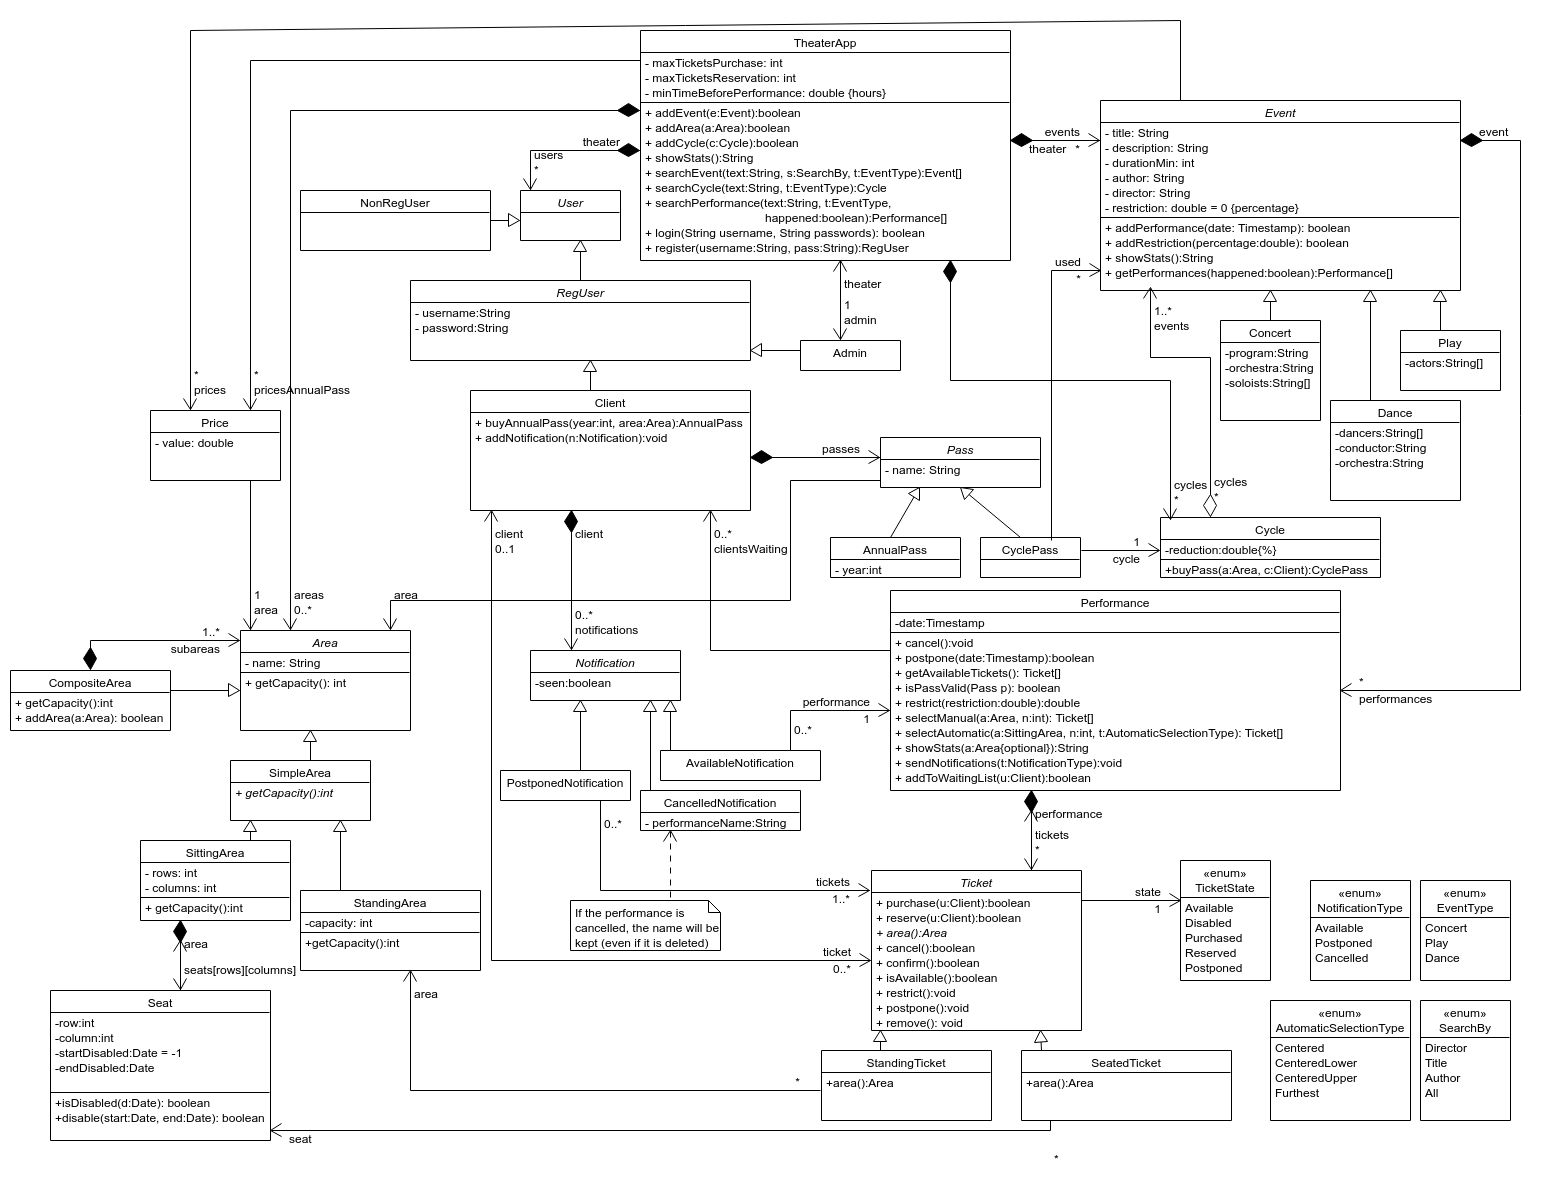
\includegraphics[scale=.2929306]{../class_diagram/ver2}
    \caption{Class diagram}
\end{figure}

The theater app contains all the information of the system. It is a container of areas (all the areas of the theater), users, cycles and events. 
It has all the methods for searching (which can be used by any user). 
Also, for adding events or areas and showing stats of the events, which can be used only by the administrator of the theater. 
As private attributes, there are parameters that can be configured by the administrator like the maximun number of tickets per reservation, or the prices of the annual passes or each area.

Event is an abstract class with subclasses (one for each kind) that have specific attributes. 
Each event contains all its performances, and performances have a list of all its tickets, each of them with an attribute that indicates its state, depending on its availability. 
To satisfy the requirements, we have included methods to add new performances to an event, as well as postponing an cancelling them.

It is worth commenting the Ticket class as it is the link between clients and performances. When a performance is created, one ticket for each available spot in the theater (standing or seated) is created. This ticket can be purchased and reserved by clients, but they may also be disabled due to restrictions or because the seat of the ticket is disabled.
The different states of this class will be explained with more detail in the state diagram.
Moving on to the areas, we have stablished again an abstract class with subclasses. In this case there is an overriden method \textit{getCapacity()} that has a different implementation for each subclass.

Finally, there are several enumeration classes in the diagram: almost all of them are used for restricting the parameter of methods. For instance, there is an enumeration for the different ways of searching
for an event (by director, title or author) and another for specifying the criteria when selecting seats in an automatic selection.



\newpage

\section{State diagrams}

\subsection{State diagram of class: \texttt{Performance}}

\begin{figure}[h]
    \centering
    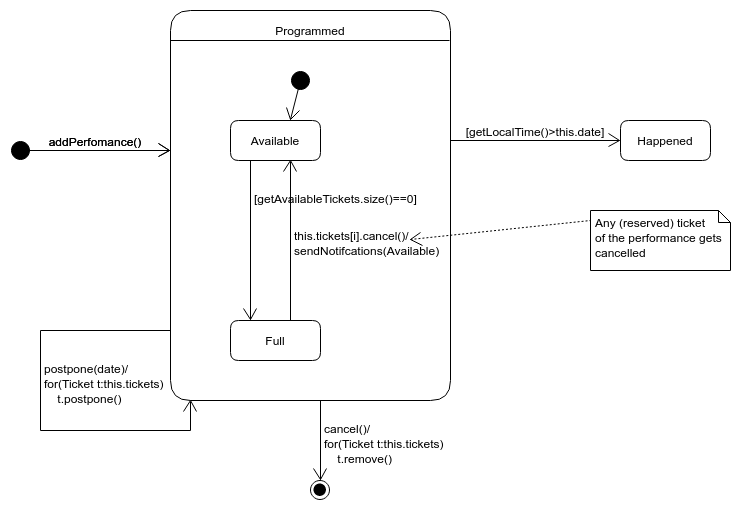
\includegraphics[width=400pt]{../state2/perf}
    \caption{State diagram: \texttt{Performance}}
\end{figure}

We have defined 2 general states: programmed and happened. In addition, an object of type performance is eliminated when the performance is cancelled (and, as a result, clients who had purchased/reserved a ticket get the appropiate notification-handled by the method \texttt{Ticket.remove()}).
\begin{itemize}
    \item \textbf{Programmed}: This is a composite state that shows that the performanced has not taken place yet. The transition to \texttt{Happened} is the same for the two atomic states inside, and implies that the scheduled date of the performance already belongs to the past. On the other hand, programmed events can be postponed, which does not result in a change of state; the method \texttt{Ticket.postpone()} is invoked over every ticket of the performance, so each client receives a notification. 
    \begin{itemize}
        \item \textbf{Available}: This is the initial state of any performance that has been created (as the diagram shows). The transition to \texttt{Full} only happens when the guard ``no empty spots'' is met (which in our design of the class performance, it can be translated into the condition that the list of available tickets is empty).
        \item \textbf{Full}: It is the opposite state of \textit{Available}, and its transition implies calling the method \textit{sendNotification(Available)} (the argument in this method specifies the type of notification that must be sent and to whom-clients in the waiting list).
    \end{itemize}
    \item \textbf{Happened}: This state is needed so it makes sense to search for ``upcoming performances'' (the complementary set), as well as being able to retrieve the stats of past performances.
\end{itemize}
\newpage

\subsection{State diagram of class: \texttt{Ticket}}

\begin{figure}[h]
    \centering
    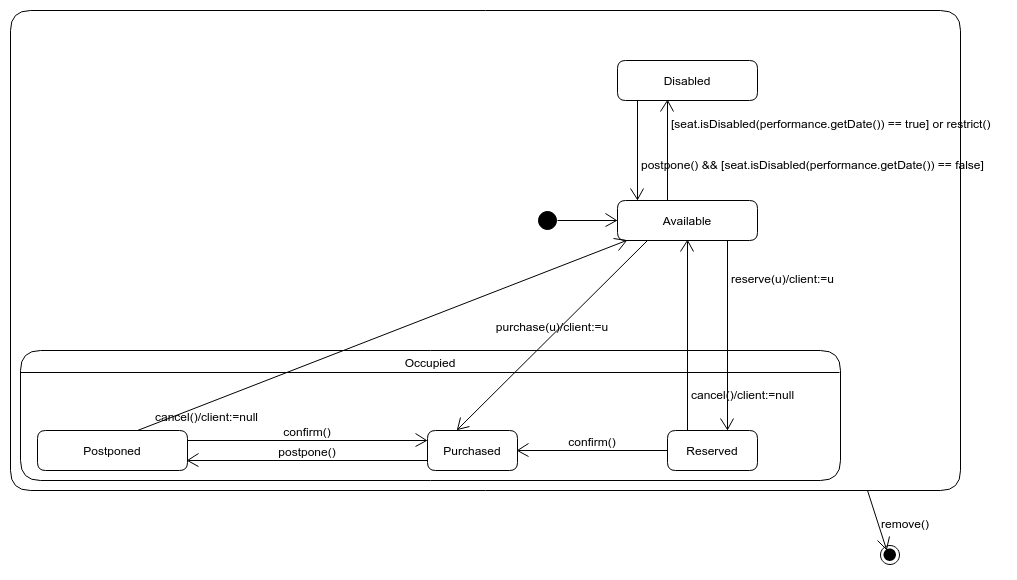
\includegraphics[width=400pt]{../state1/s1}
    \caption{State diagram: \texttt{Ticket}}\label{state1}
\end{figure}

This class has 5 possible states:
\begin{itemize}
    \item \textbf{Available}: The default state, when a performance is created all tickets are available (unless they correspond to a seat that is disabled). If a ticket is cancelled (from Reserved or Postponed), it becomes available.
    \item \textbf{Disabled}: This is the state of the disabled seats. Also, if the admin has applied a restriction to an event, the restricted seats (calculated automatically) will also be in this state.
    \item \textbf{Occupied}: the ticket is associated with a user (composite state):
    \begin{itemize}
        \item \textbf{Reserved}: When the ticket has been reserved by a user. 
        \item \textbf{Purchased}: When the ticket has been bought by a user, or a reservation (or postponed ticket) is confirmed.
        \item \textbf{Postponed}: This state is reached when the performance is postponed and the ticket was purchased. In this state, the client can confirm the ticket or cancel it (getting their money back). If the client does none of this things, the ticket counts as Purchased when the expiration time is reached.
    \end{itemize}
\end{itemize}

Note on \texttt{postpone()}: This method appears in two of the transitions of the diagram (\ref{state1}). It means that, when the performance is postponed, it will invoke this method over all of its tickets and modify their state if necessary: disabled tickets could become available if they are not disabled in the new date, and purchased tickets become \textit{postponed}. If necessary, notificatios to the clients will also be sent.

\texttt{remove()} is a method that is invoked over all of the tickets when the performace is cancelled, after this method, the ticket will be removed. Depending on its state, this method will send notifications to the client, or give the money back.


\newpage



\section{Sequence diagrams}

\subsection{Sequence diagram: Create area (configure areas)}

\begin{figure}[h]
    \centering
    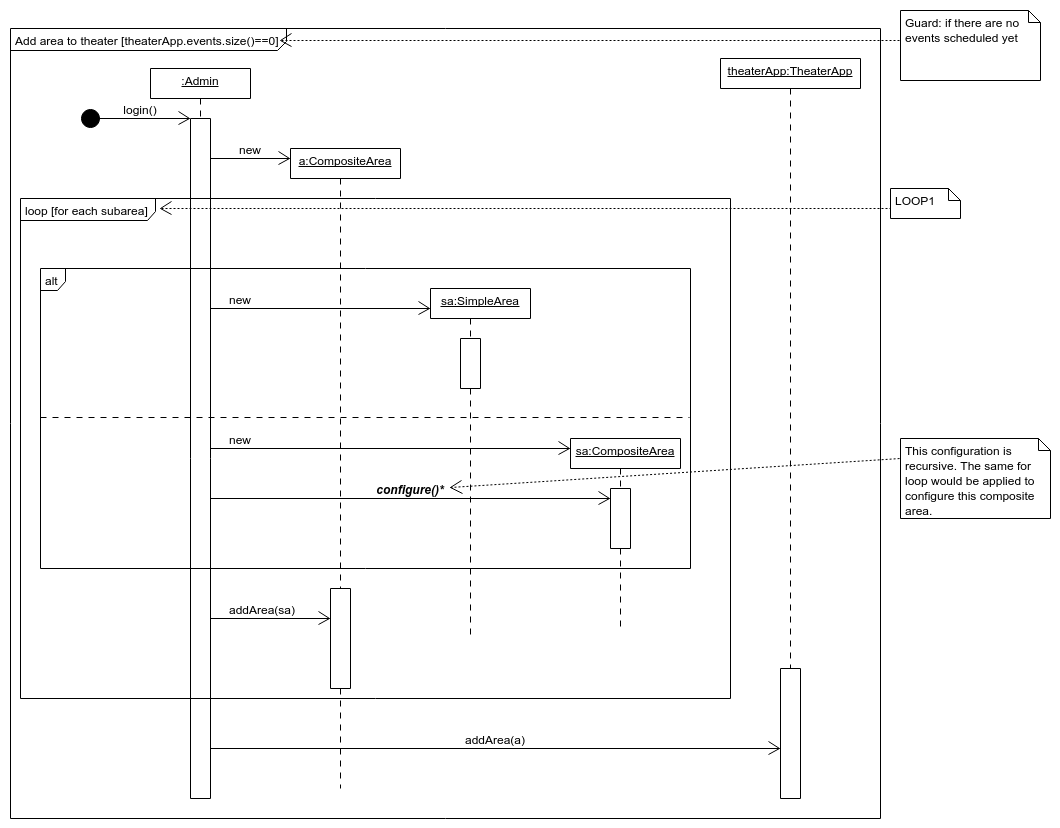
\includegraphics[width=450pt]{../sequence_area/addArea}
    \caption{State diagram: \texttt{Ticket}}\label{seq}
\end{figure}

The administrator, after logging in, can create a composite area inside the theater. Then there is a loop (the configuration of that area) where all of the subareas are added. The subareas can be of two types (alternate path): composite or simple. The simple subareas are just created. The composite subareas have to be configured with a loop (the configuration of the area) just like  \texttt{LOOP1} in Figure \ref{seq}. Each created subarea has to be added to the composite area.

Finally the composite area that has been created is added to the areas of the Theater.

Of course, this action can only be performed when there are no events in the system.

\newpage

\subsection{Sequence diagram: Purchase/Reserve tickets}

\begin{figure}[ht]
    \centering
    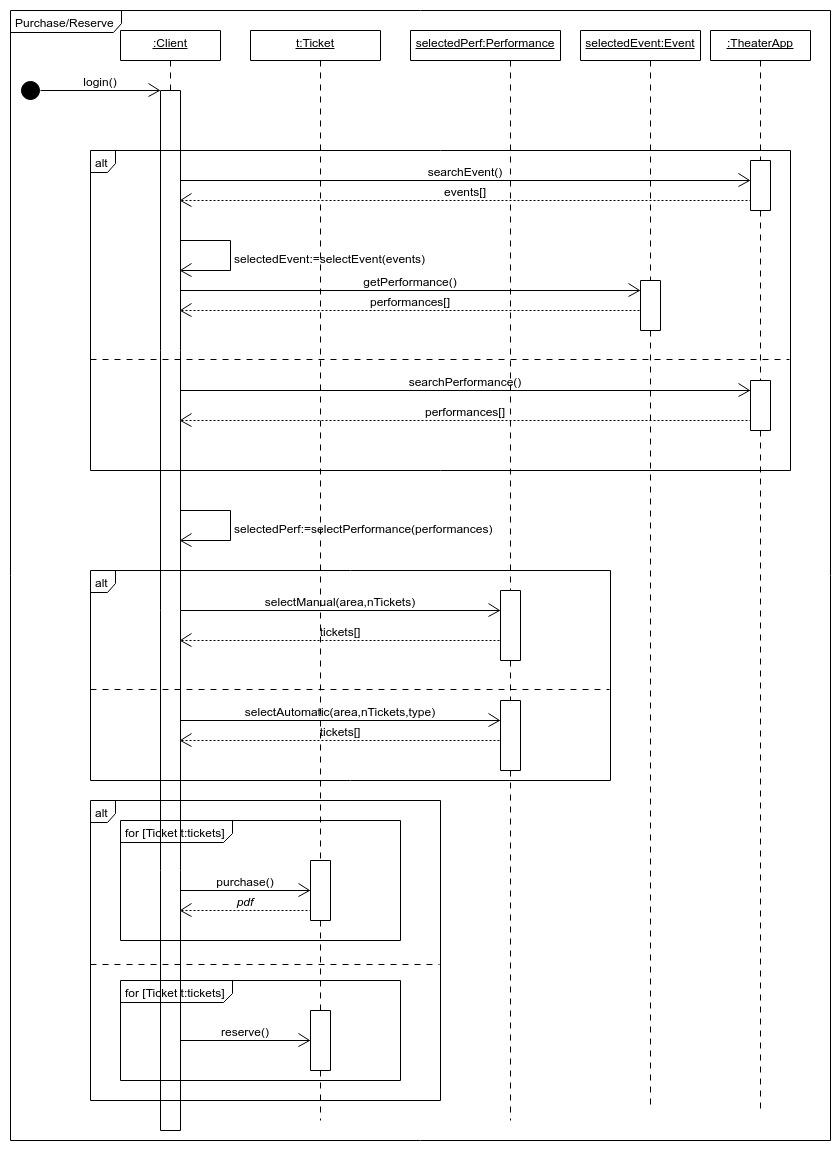
\includegraphics[width=380pt]{../sequence_buy/buy}
    \caption{Sequence diagram: Purchase/Reserve tickets}
\end{figure}

This action (purchase or reserve) can only be made by Clients.
Firstly, the client selects a performance. There are two ways of selecting a performance: by searching the event and then selecting the performance, or by directly searching performances.

In second place, the client has to select the tickets automatically or manually. 
Finally, the client selects whether to buy the tickets or reserve them. If the tickets are purchased, a pdf is generated with an authentication code.

\newpage

\section{Requirements traceability matrix}

\begin{figure}[h!]
    \centering
    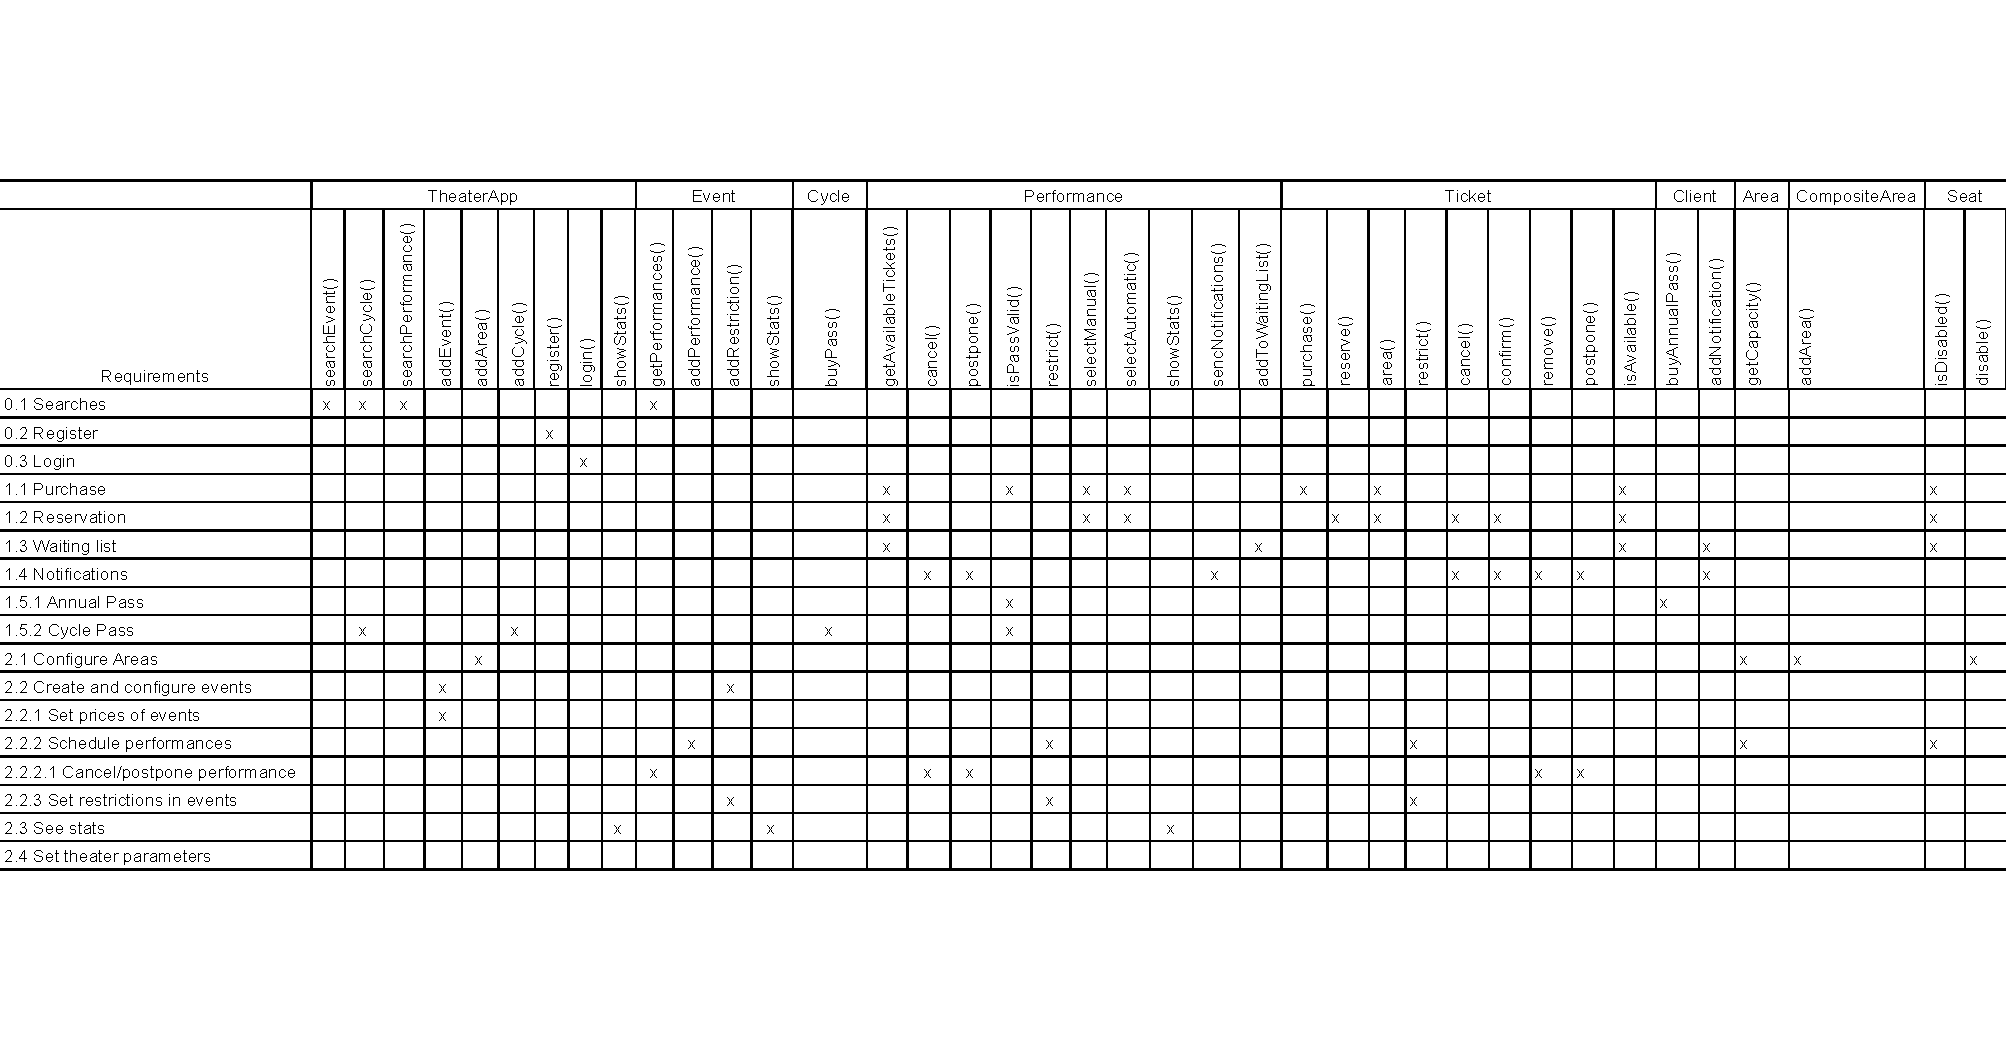
\includegraphics[width=455pt]{../matrix/matrix}
    \caption{Requirements traceability matrix}
\end{figure}

The matrix above shows how the different funcionalities specified in the RAD (Requirement Analysis Document) are solved by the methods of each class. For simplycity sake, most getters and setters have not been included. Finally, we would like to mention that the funcionality ``Set theater parameters'' (2.4), is met mainly with getters of the \textit{TheaterApp} class which are not in the matrix.






\end{document}
